\subsection{System Call Invocation Frequencies}
To determine what calls were invoked most frequently by programs, we used \texttt{strace} and \texttt{ltrace} to monitor library and system calls, respectively. We ran each of the small-scale utilities listed in tables \ref{lst:coreutils}, \ref{lst:net-tools}, and \ref{lst:other_utilities} (excluding \texttt{man} and \texttt{ssh}) once. These utilities represent a sizable sample of the programs commonly used by a systems programmer. Bar charts showing the system call counts and library call counts observed are shown in figures \ref{fig:sys_counts} and \ref{fig:lib_counts}, respectively. Among the most frequently called, many have a return type of \texttt{void} and therefore do not fit within our return value testing framework.\\
%Another set was determined to be false positives, due to the numerous setup calls which occur before the actual program code begins executing (e.g. \texttt{mmap}). \\
\begin{figure}
\centering
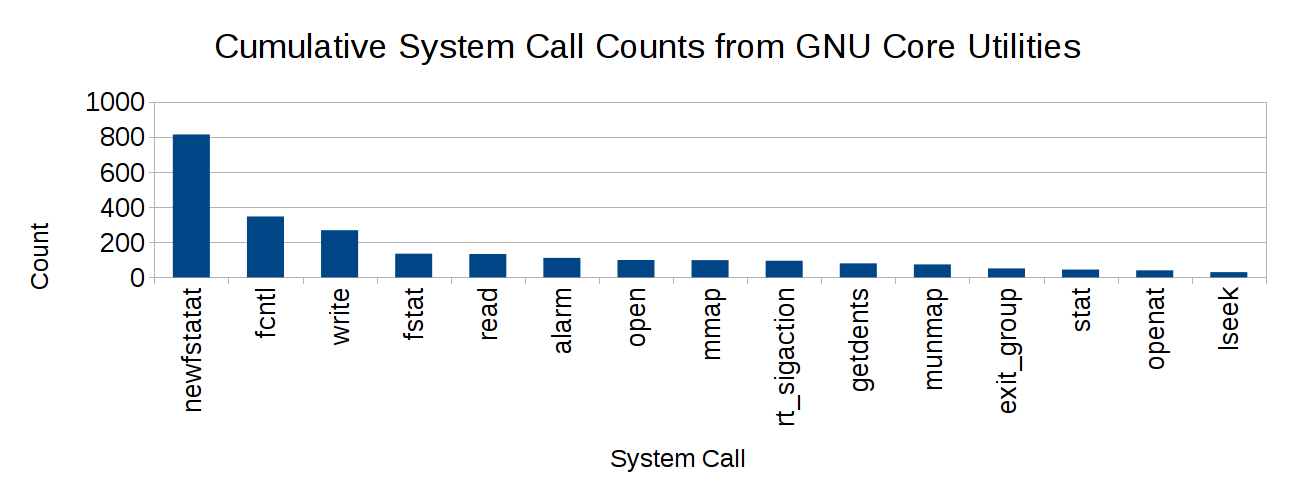
\includegraphics[width=\textwidth]{sys_counts}
\caption{Most frequently invoked system calls in a sample run of common utilities}
\label{fig:sys_counts}
\end{figure}

\begin{figure}
\centering
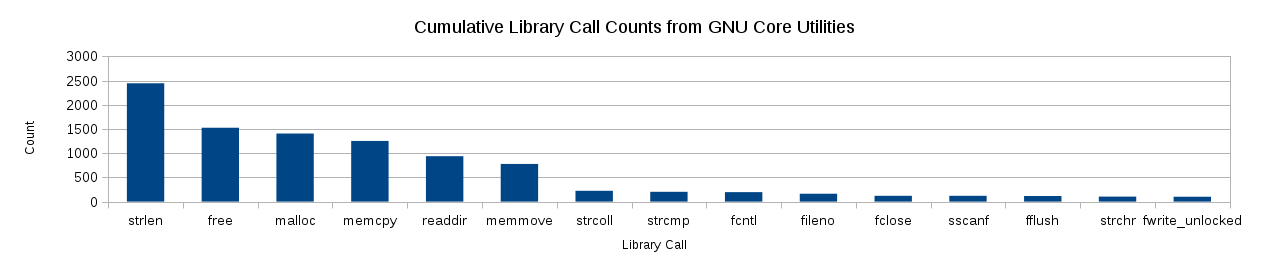
\includegraphics[width=\textwidth]{lib_counts}
\caption{Most frequently invoked library calls in a sample run of common utilities}
\label{fig:lib_counts}
\end{figure}
